\documentclass[12pt]{article}
\usepackage{amsmath}
\usepackage{amssymb}
\usepackage[letterpaper,margin=0.85in,centering]{geometry}
\usepackage{fancyhdr}
\usepackage{enumerate}
\usepackage{lastpage}
\usepackage{multicol}
\usepackage{graphicx}

\reversemarginpar

\pagestyle{fancy}
\cfoot{}
\lhead{Math 2560}\chead{Worksheet \# 5}\rhead{Thursday 25\textsuperscript{th} February, 2016}
%\rfoot{Total: 10 points}
%\chead{{\bf Name:}}
\newcommand{\points}[1]{\marginpar{\hspace{24pt}[#1]}}
\newcommand{\skipline}{\vspace{12pt}}
%\renewcommand{\headrulewidth}{0in}
\headheight 30pt

\newcommand{\di}{\displaystyle}
\newcommand{\abs}[1]{\lvert #1\rvert}
\newcommand{\len}[1]{\lVert #1\rVert}
\renewcommand{\i}{\mathbf{i}}
\renewcommand{\j}{\mathbf{j}}
\renewcommand{\k}{\mathbf{k}}
\newcommand{\R}{\mathbb{R}}
\newcommand{\aaa}{\mathbf{a}}
\newcommand{\bbb}{\mathbf{b}}
\newcommand{\ccc}{\mathbf{c}}
\newcommand{\dotp}{\boldsymbol{\cdot}}
\newcommand{\bbm}{\begin{bmatrix}}
\newcommand{\ebm}{\end{bmatrix}}                   
                  
\begin{document}


%\author{Instructor: Sean Fitzpatrick}
\thispagestyle{fancy}
%\noindent{{\bf Name and student number:}}

\begin{enumerate}
 \item Find the volume of the solid generated by revolving the region bounded by $y=x^2$, $x=1$, and $y=0$ about the $x$-axis.

\begin{center}
 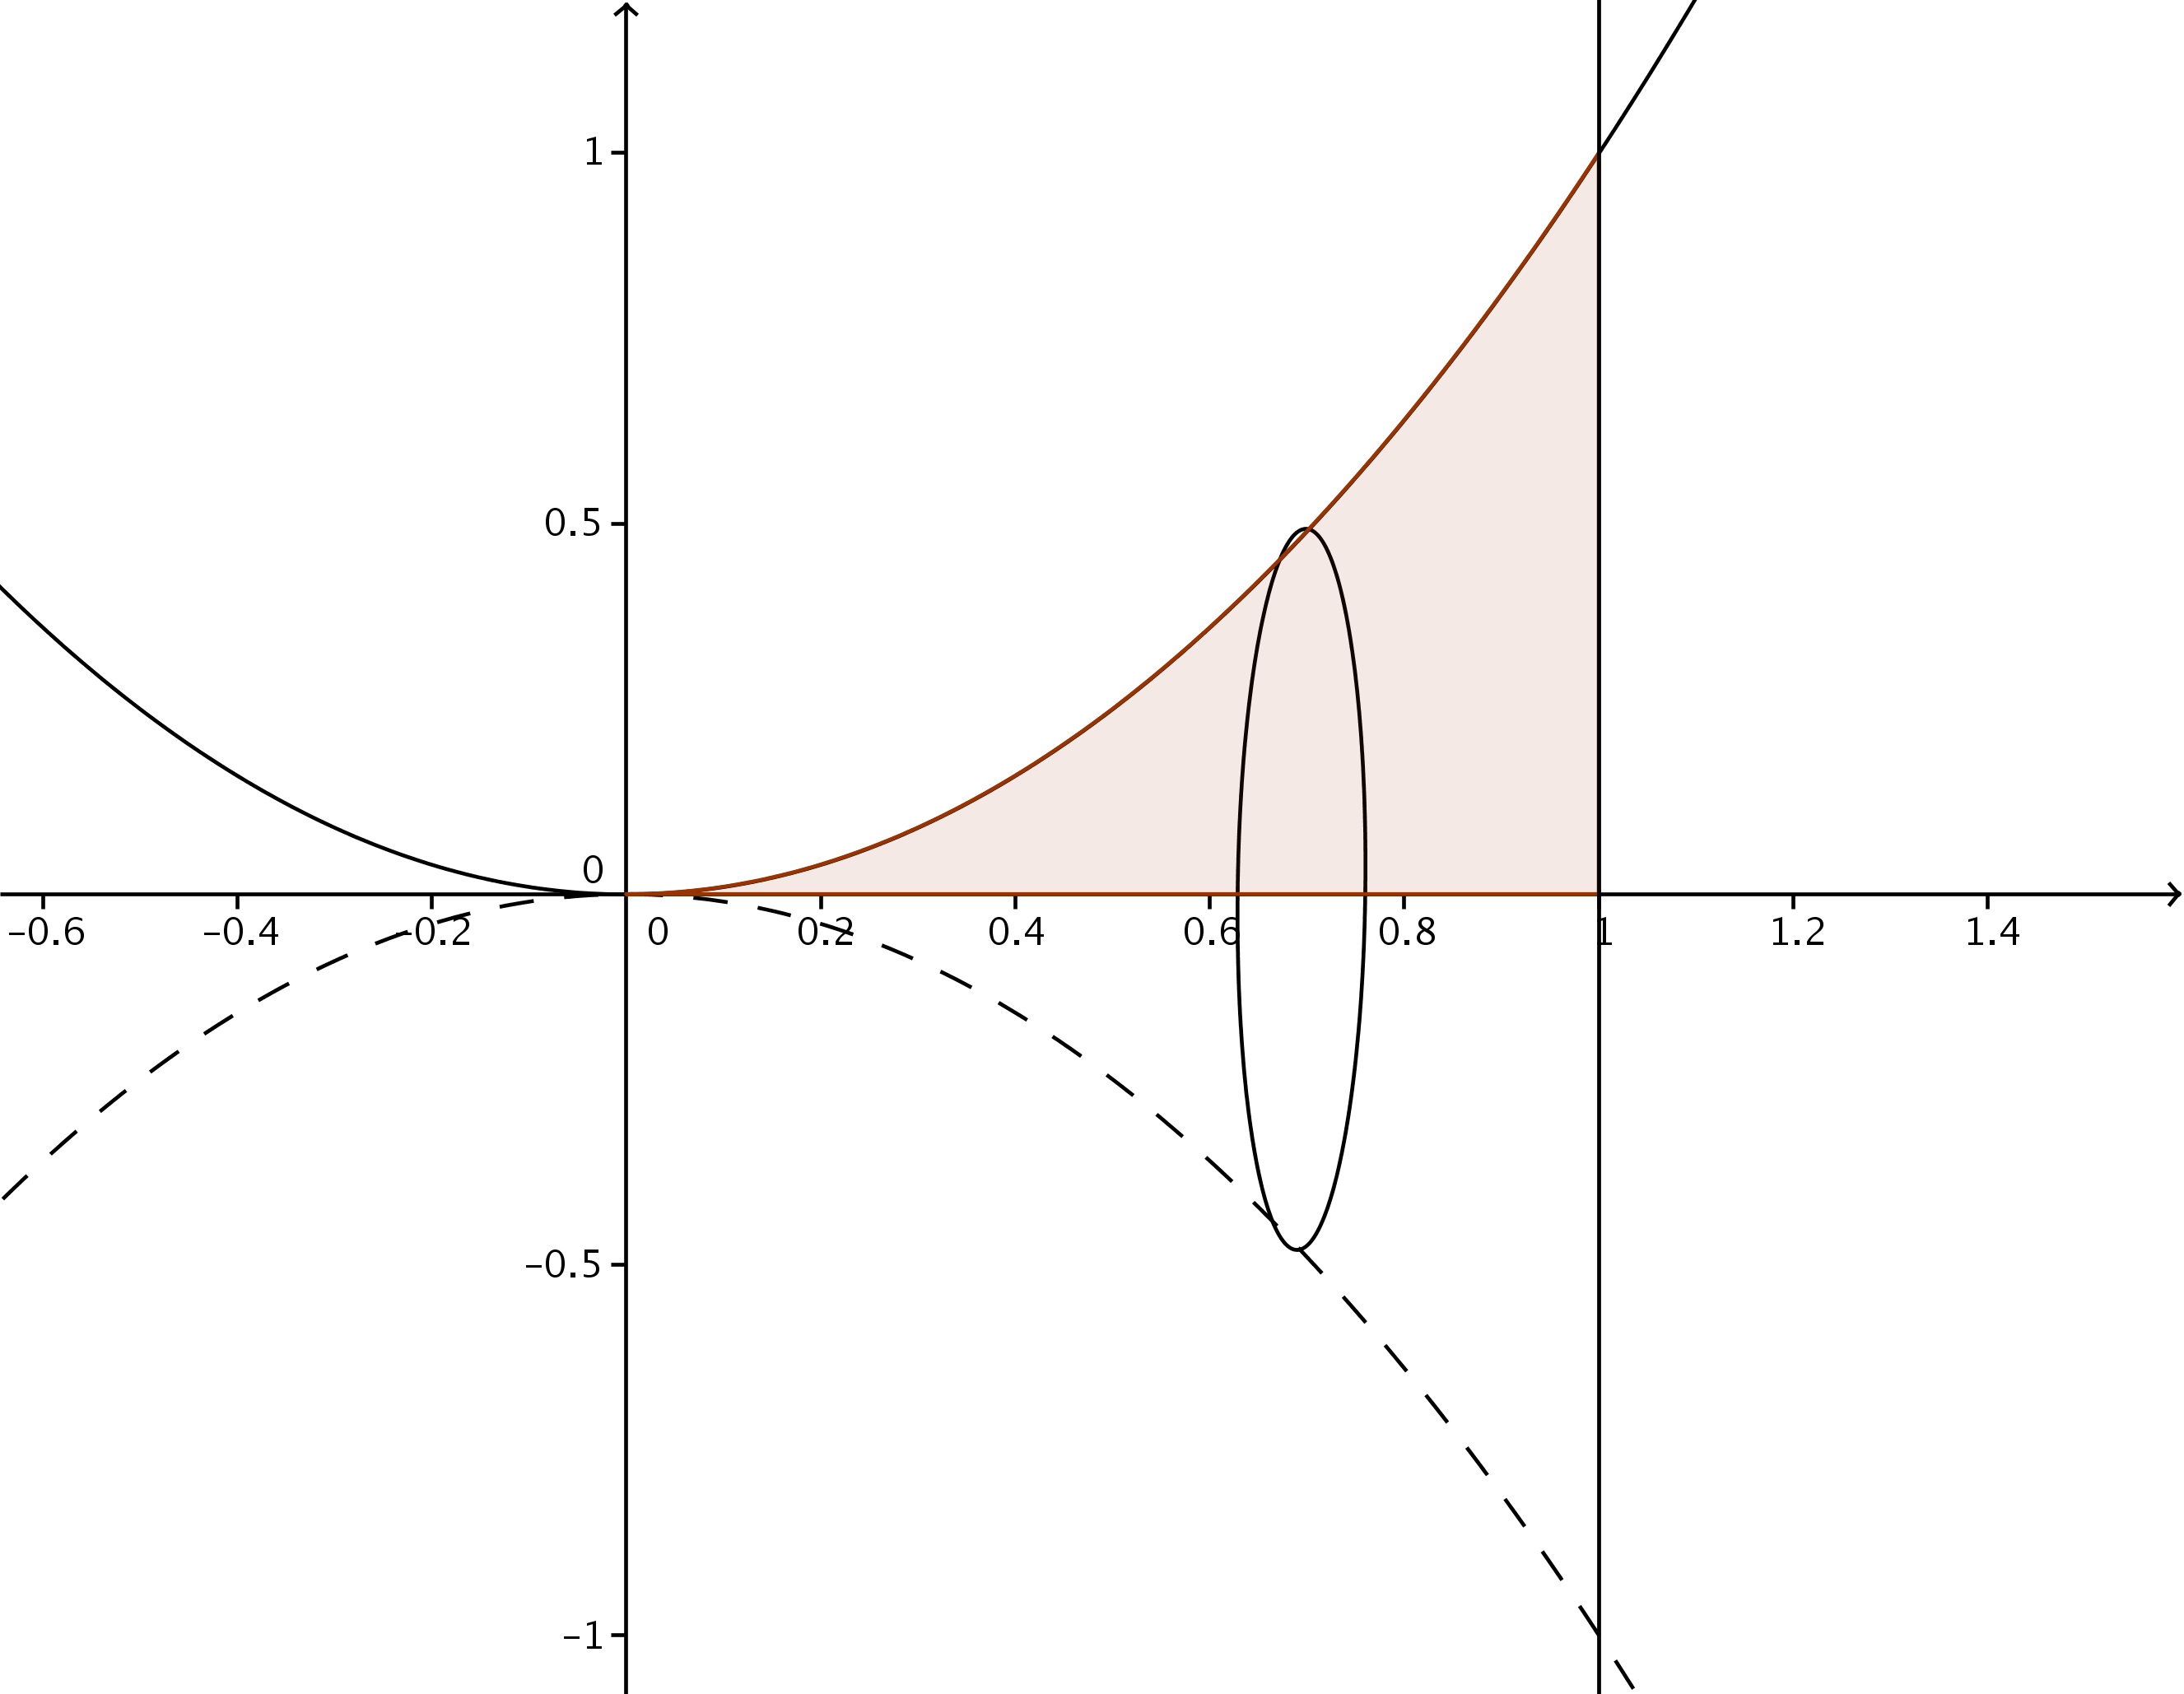
\includegraphics[width=0.5\textwidth]{WS5-1.png}
\end{center}

Using the disc method, our cross-sectional area is $A(x) = \pi y^2 = \pi(x^2)^2 = \pi x^4$. The volume is therefore
\[
 V = \int_0^1 \pi x^4\,dx = \frac{\pi}{5}.
\]

 \item Find the volume of the solid generated by revolving the region bounded by $y=\sqrt{x}$, $y=1$, and $x=0$ about the $x$-axis.

\begin{multicols}{2}
 \begin{center}
  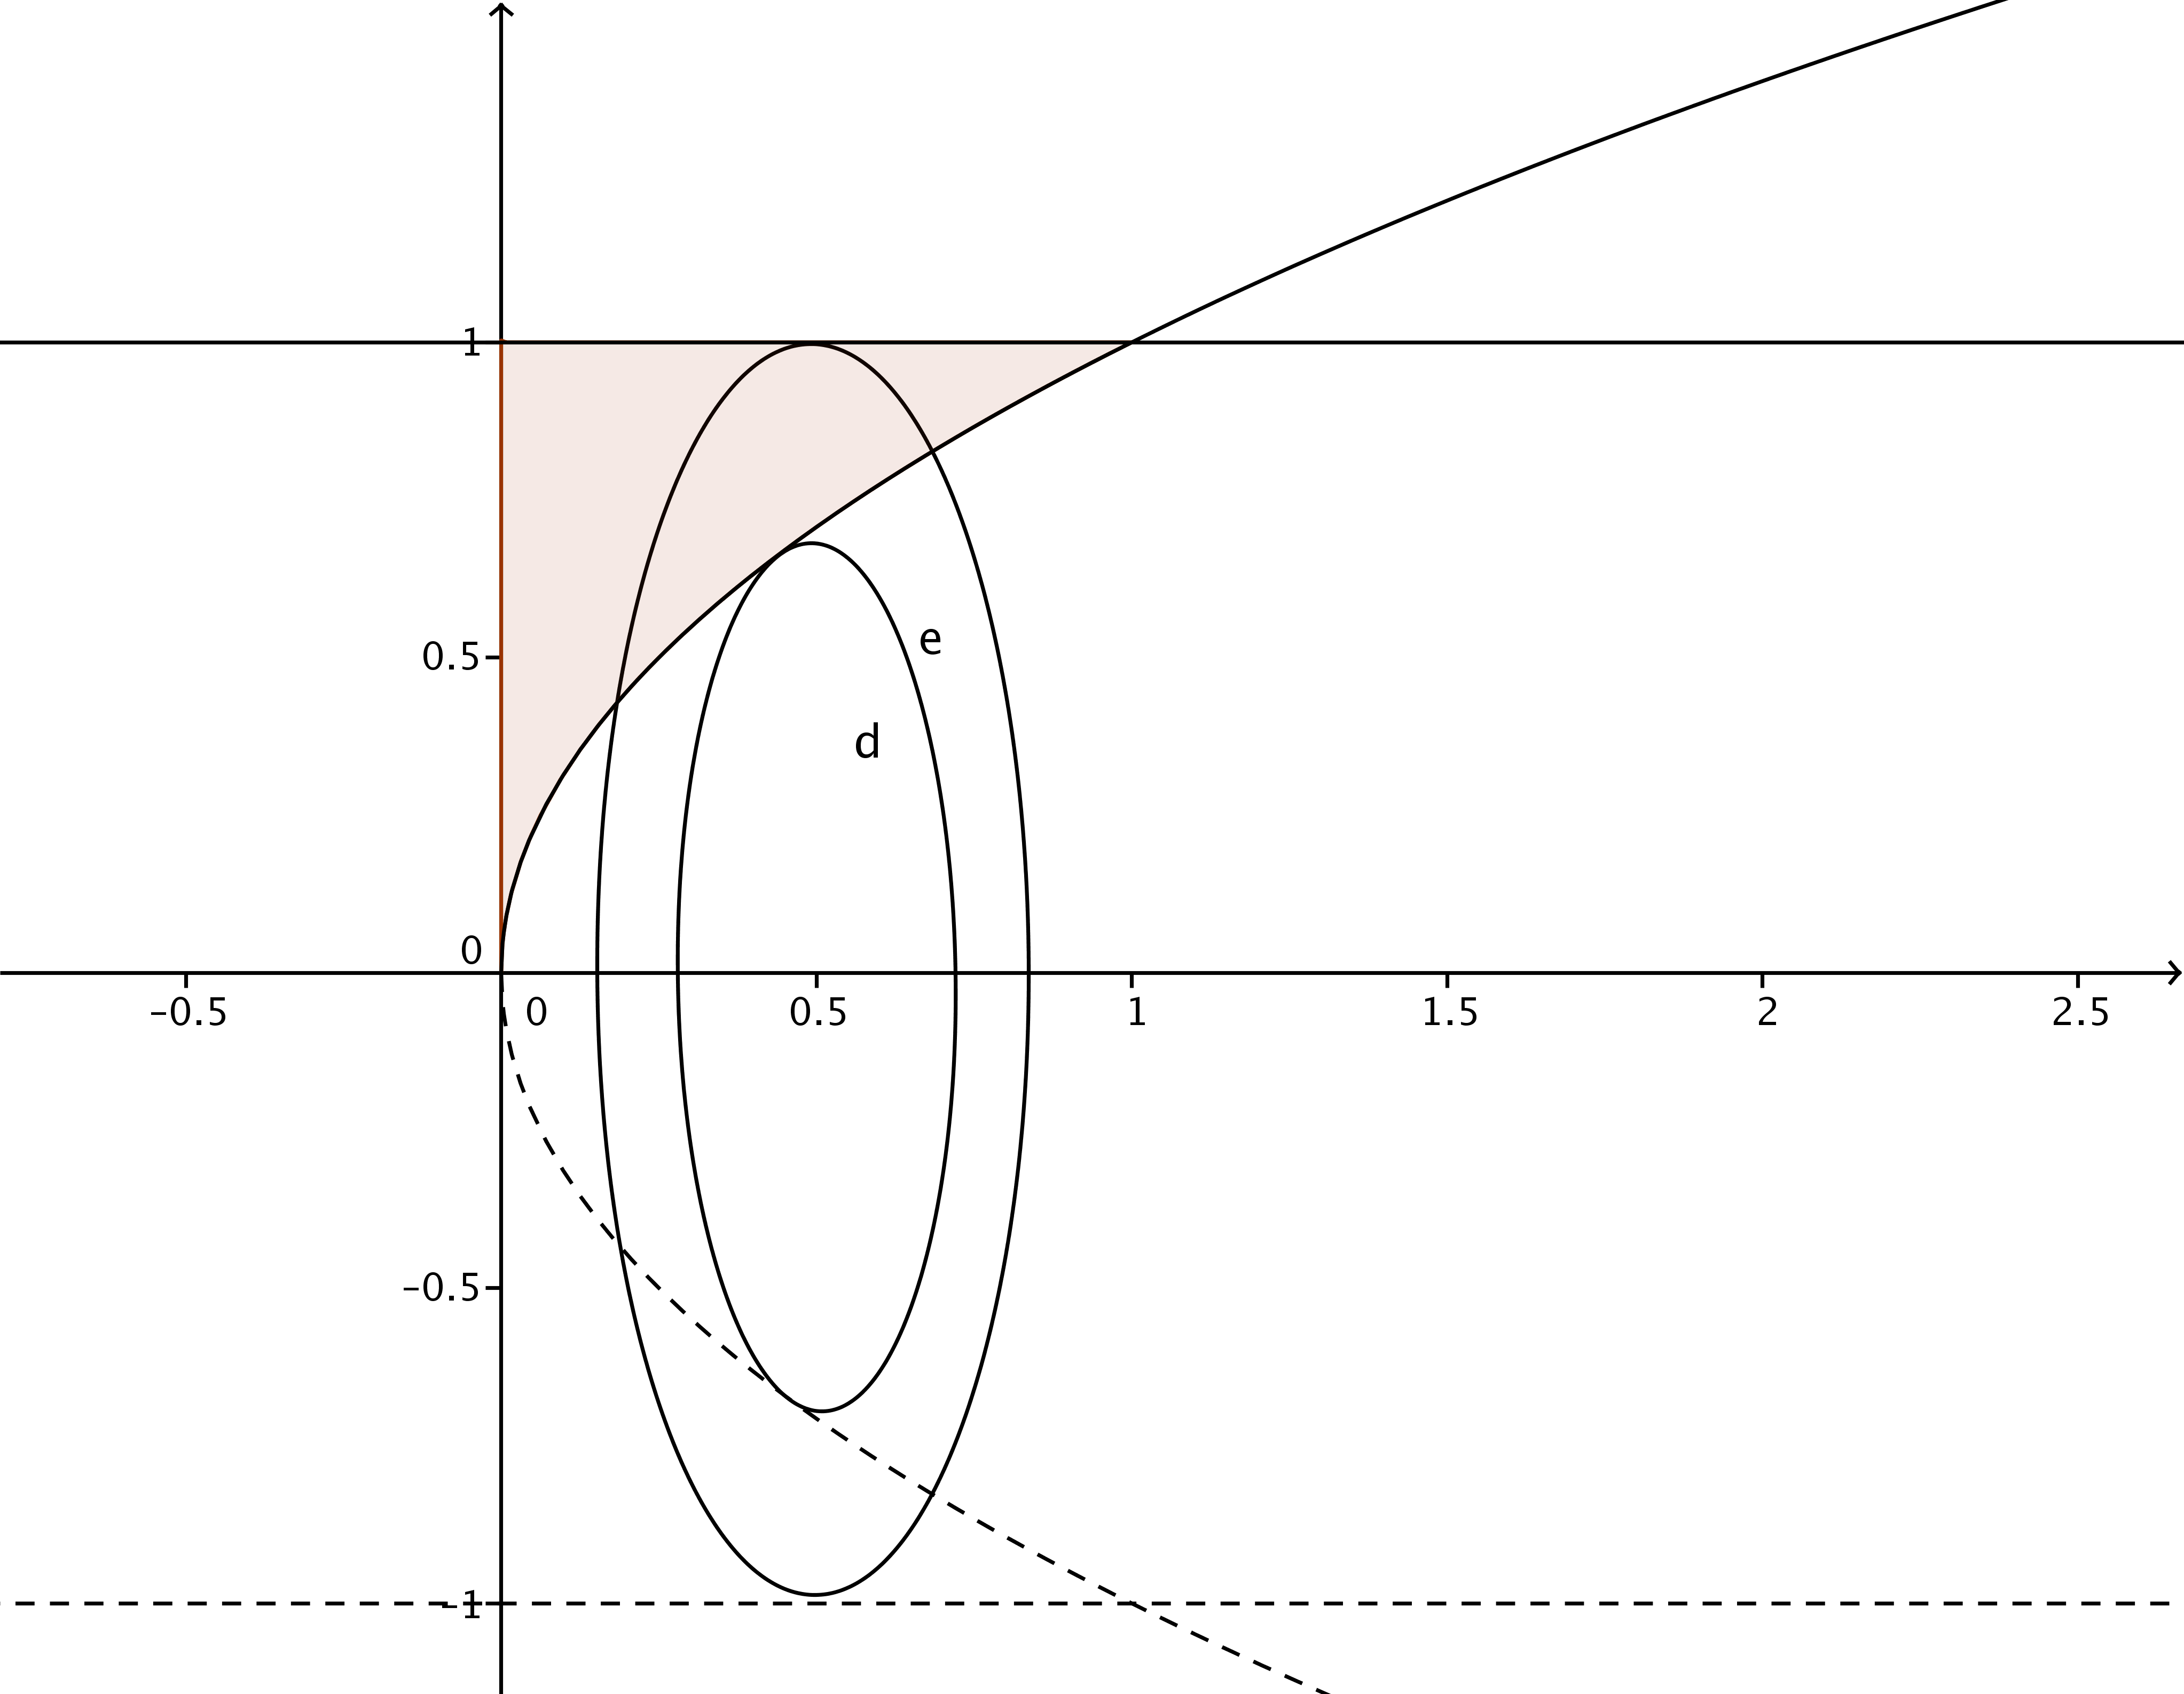
\includegraphics[width=0.8\columnwidth]{WS5-2a.png}
 \end{center}
 \begin{center}
  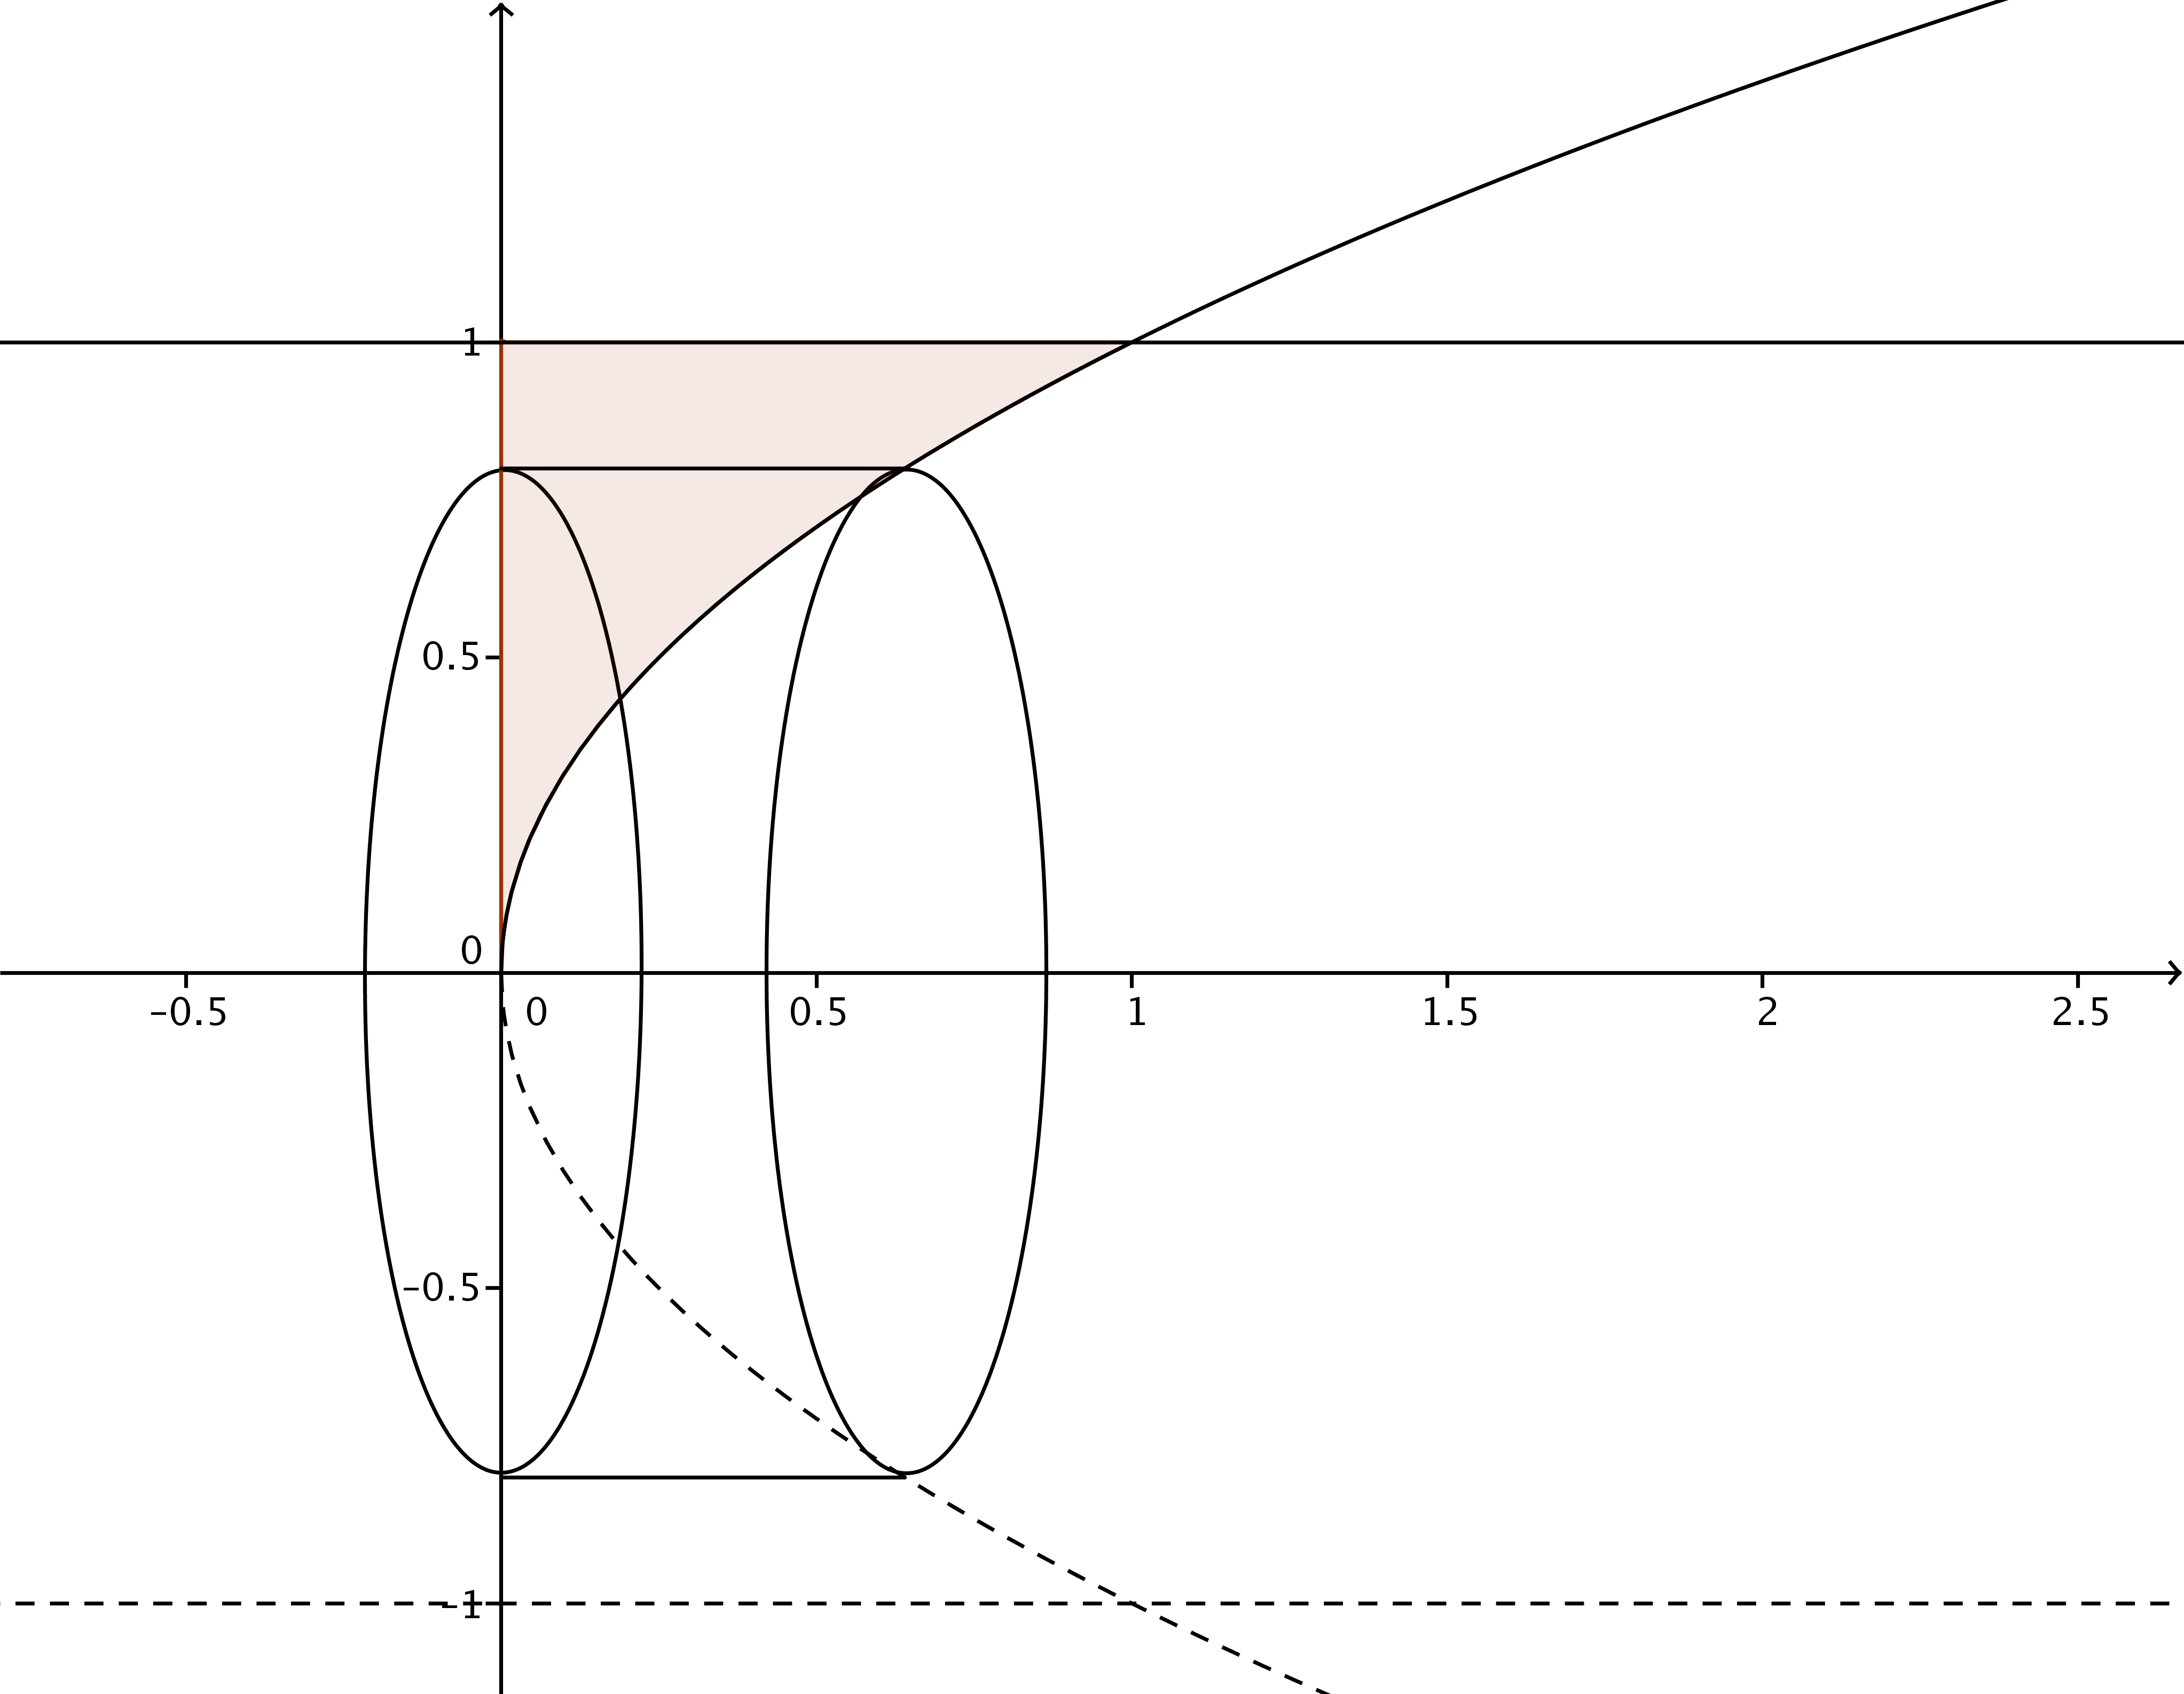
\includegraphics[width=0.8\columnwidth]{WS5-2b.png}
 \end{center}
\end{multicols}
Using washers, our cross-sectional area is $A(x) = \pi(1)^2-\pi(\sqrt{x})^2 = \pi(1-x)$, so the volume is
\[
 V = \int_0^1\pi(1-x)\,dx = \frac{\pi}{2}.
\]
If we use cylindrical shells instead, each shell has surface area $A(y) = 2\pi r(y)h(y) = 2\pi y(y^2) = 2\pi y^3$, so the volume is
\[
 V = \int_0^1 2\pi y^3\,dy = \frac{\pi}{2}.
\]

 \item Repeat Problem 2, but revolving about the $y$-axis.

\medskip

The resulting solid is identical to the one in problem 1, except that it's revolved around the $y$-axis instead of the $x$-axis, and the volume is again $\pi/5$.

 \item Find the volume of the solid generated by revolving the region bounded by $x=y-y^2$ and $x=0$ about the $y$-axis.
\begin{center}
 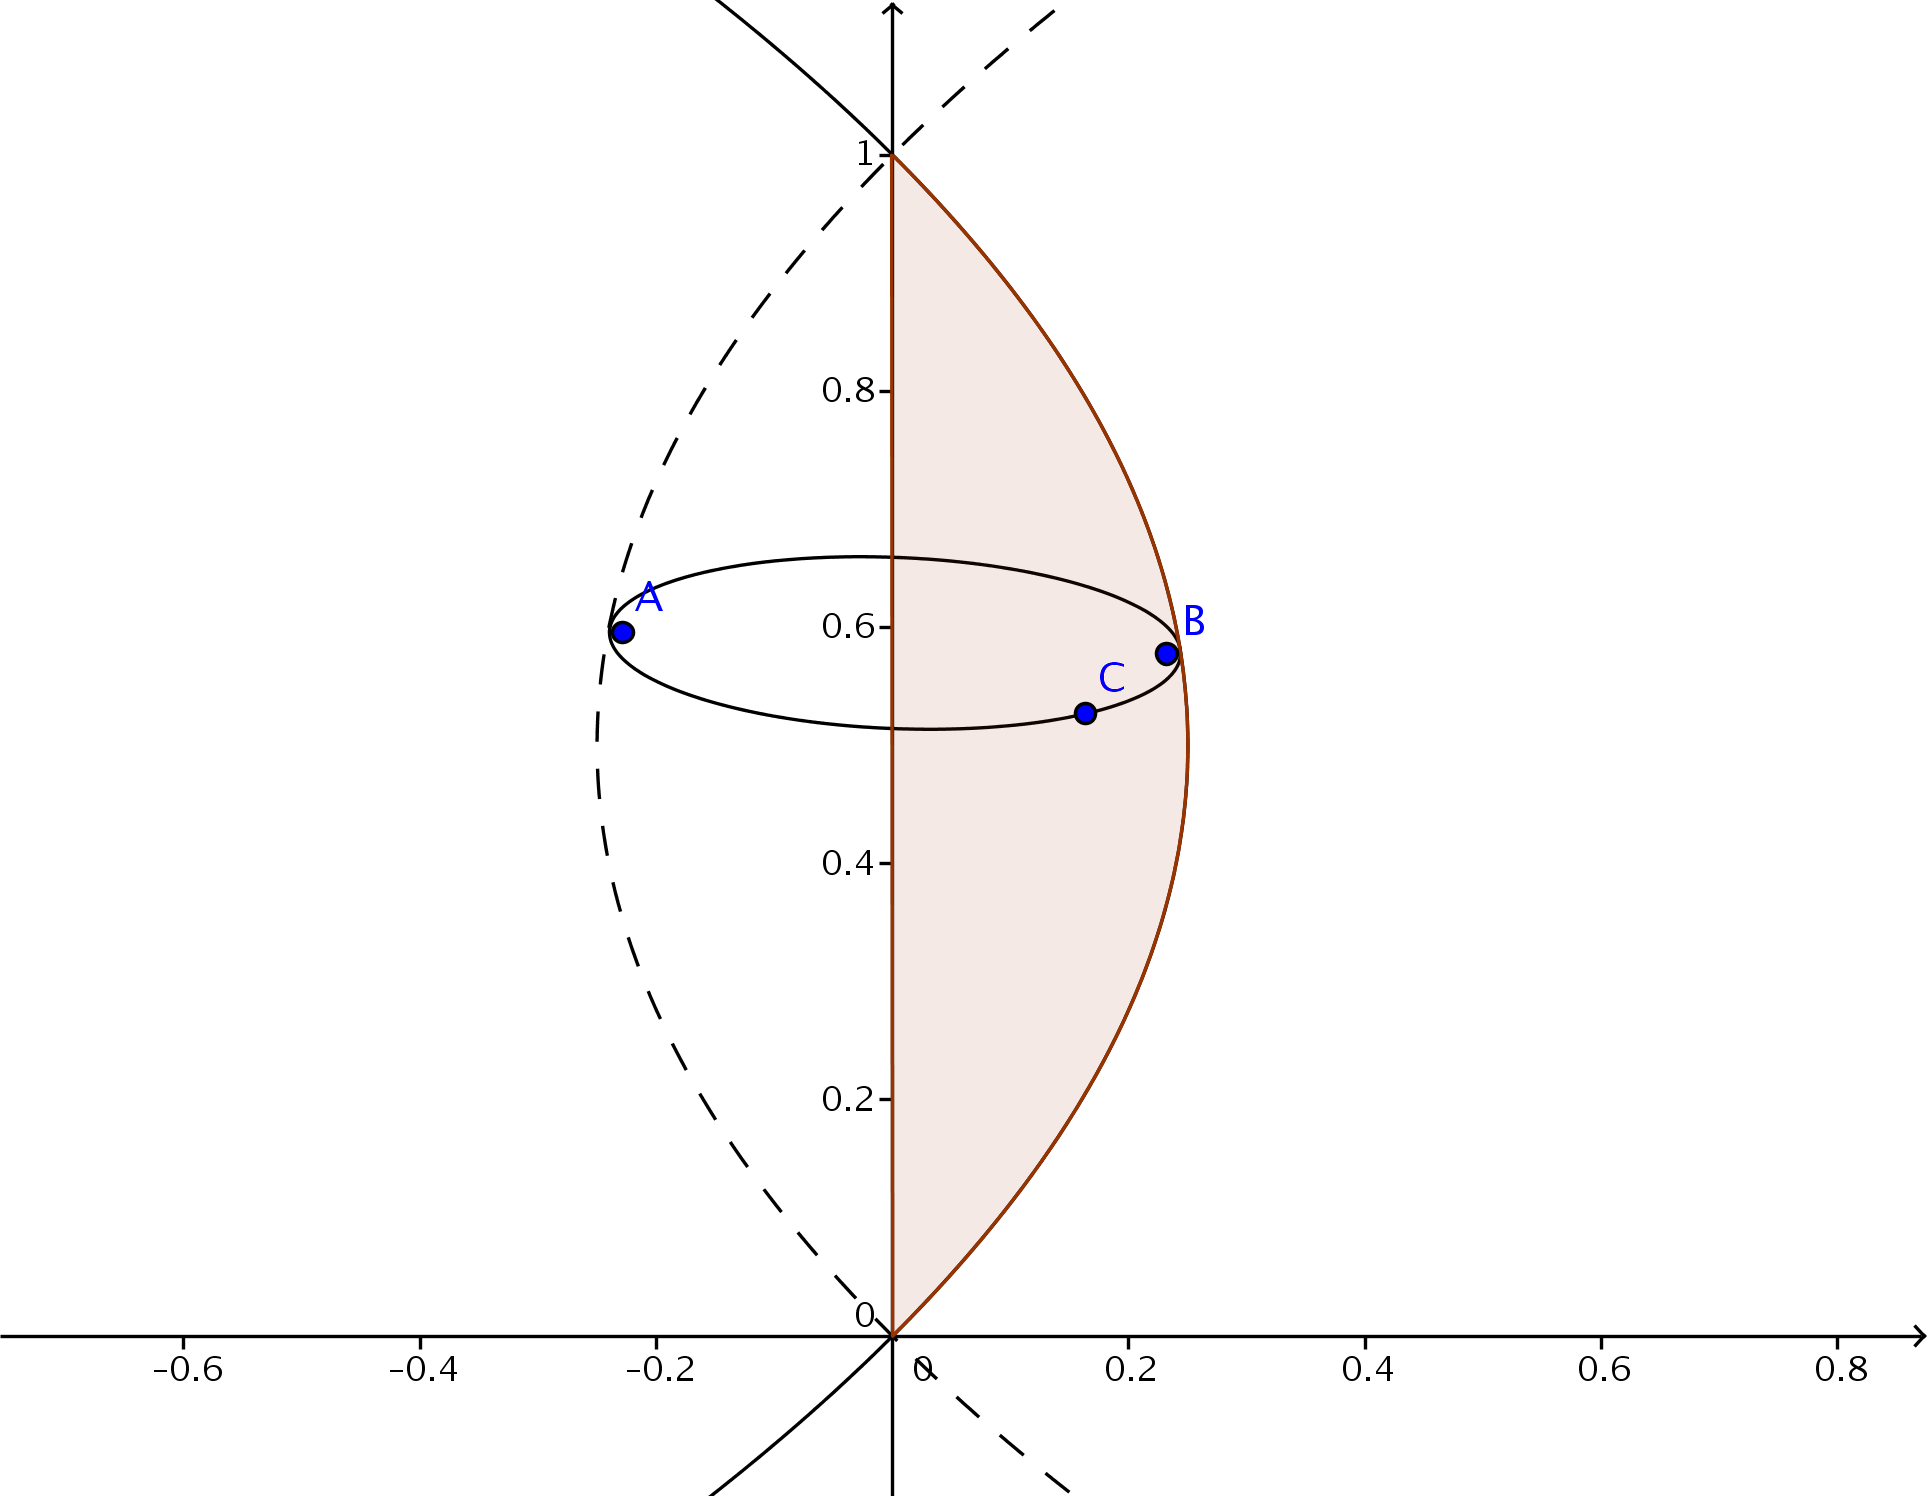
\includegraphics[width=0.5\textwidth]{WS5-4.png}
\end{center}

Using discs, we have cross-sectional area $A(y) = \pi(y-y^2)^2$, so the volume is
\[
 V = \int_0^1 \pi(y^2-2y^3+y^4)\,dy = \frac{\pi}{30}.
\]


 \item Use the shell method to find the volume of the solid generated by revolving the region bounded by $y=6x-2x^2$ and $y=0$, about the $y$-axis.

\begin{center}
 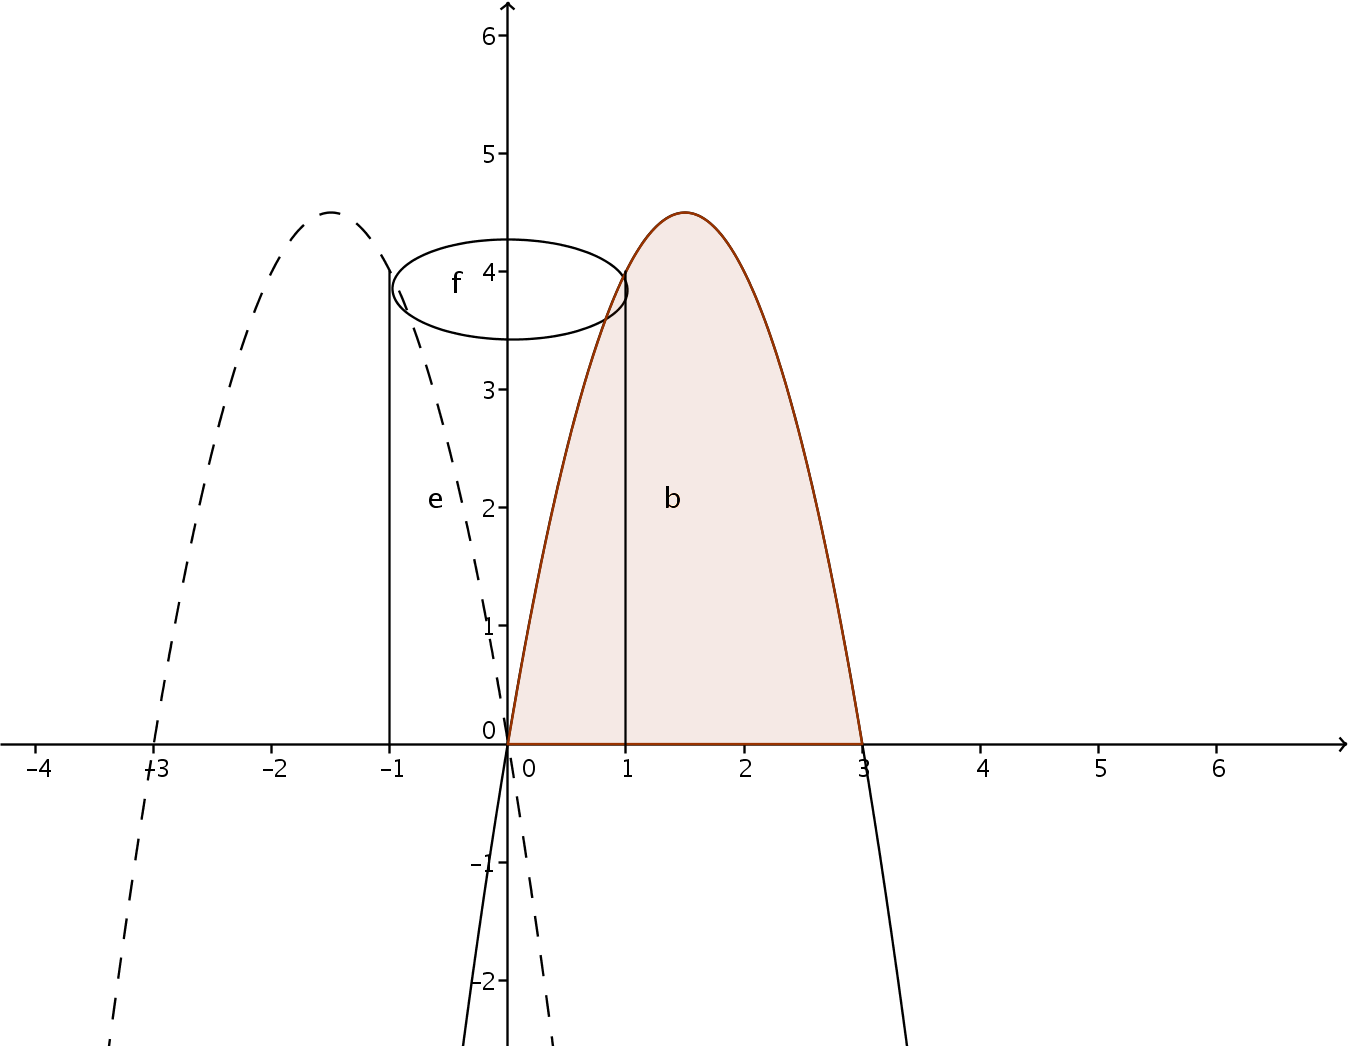
\includegraphics[width=0.5\textwidth]{WS5-5.png}
\end{center}

Note that $6x-2x^2=2x(3-x)$, so the graph $y=6x-2x^2$ intersects the $x$-axis when $x=0$ and $x=3$. Using shells, the height of each cylinder is $h = y = 6x-2x^2$, and the radius is $r=x$, so the surface area of each shell is $2\pi x(6x-2x^2)$, and the volume is
\[
 V = \int_0^3 2\pi x(6x-2x^2)\,dx  = 27\pi.
\]

 \item Use the shell method to find the volume of the solid generated by revolving the region bounded by $y=x$ and $y=\sqrt{x}$ about the $x$-axis.
\begin{center}
 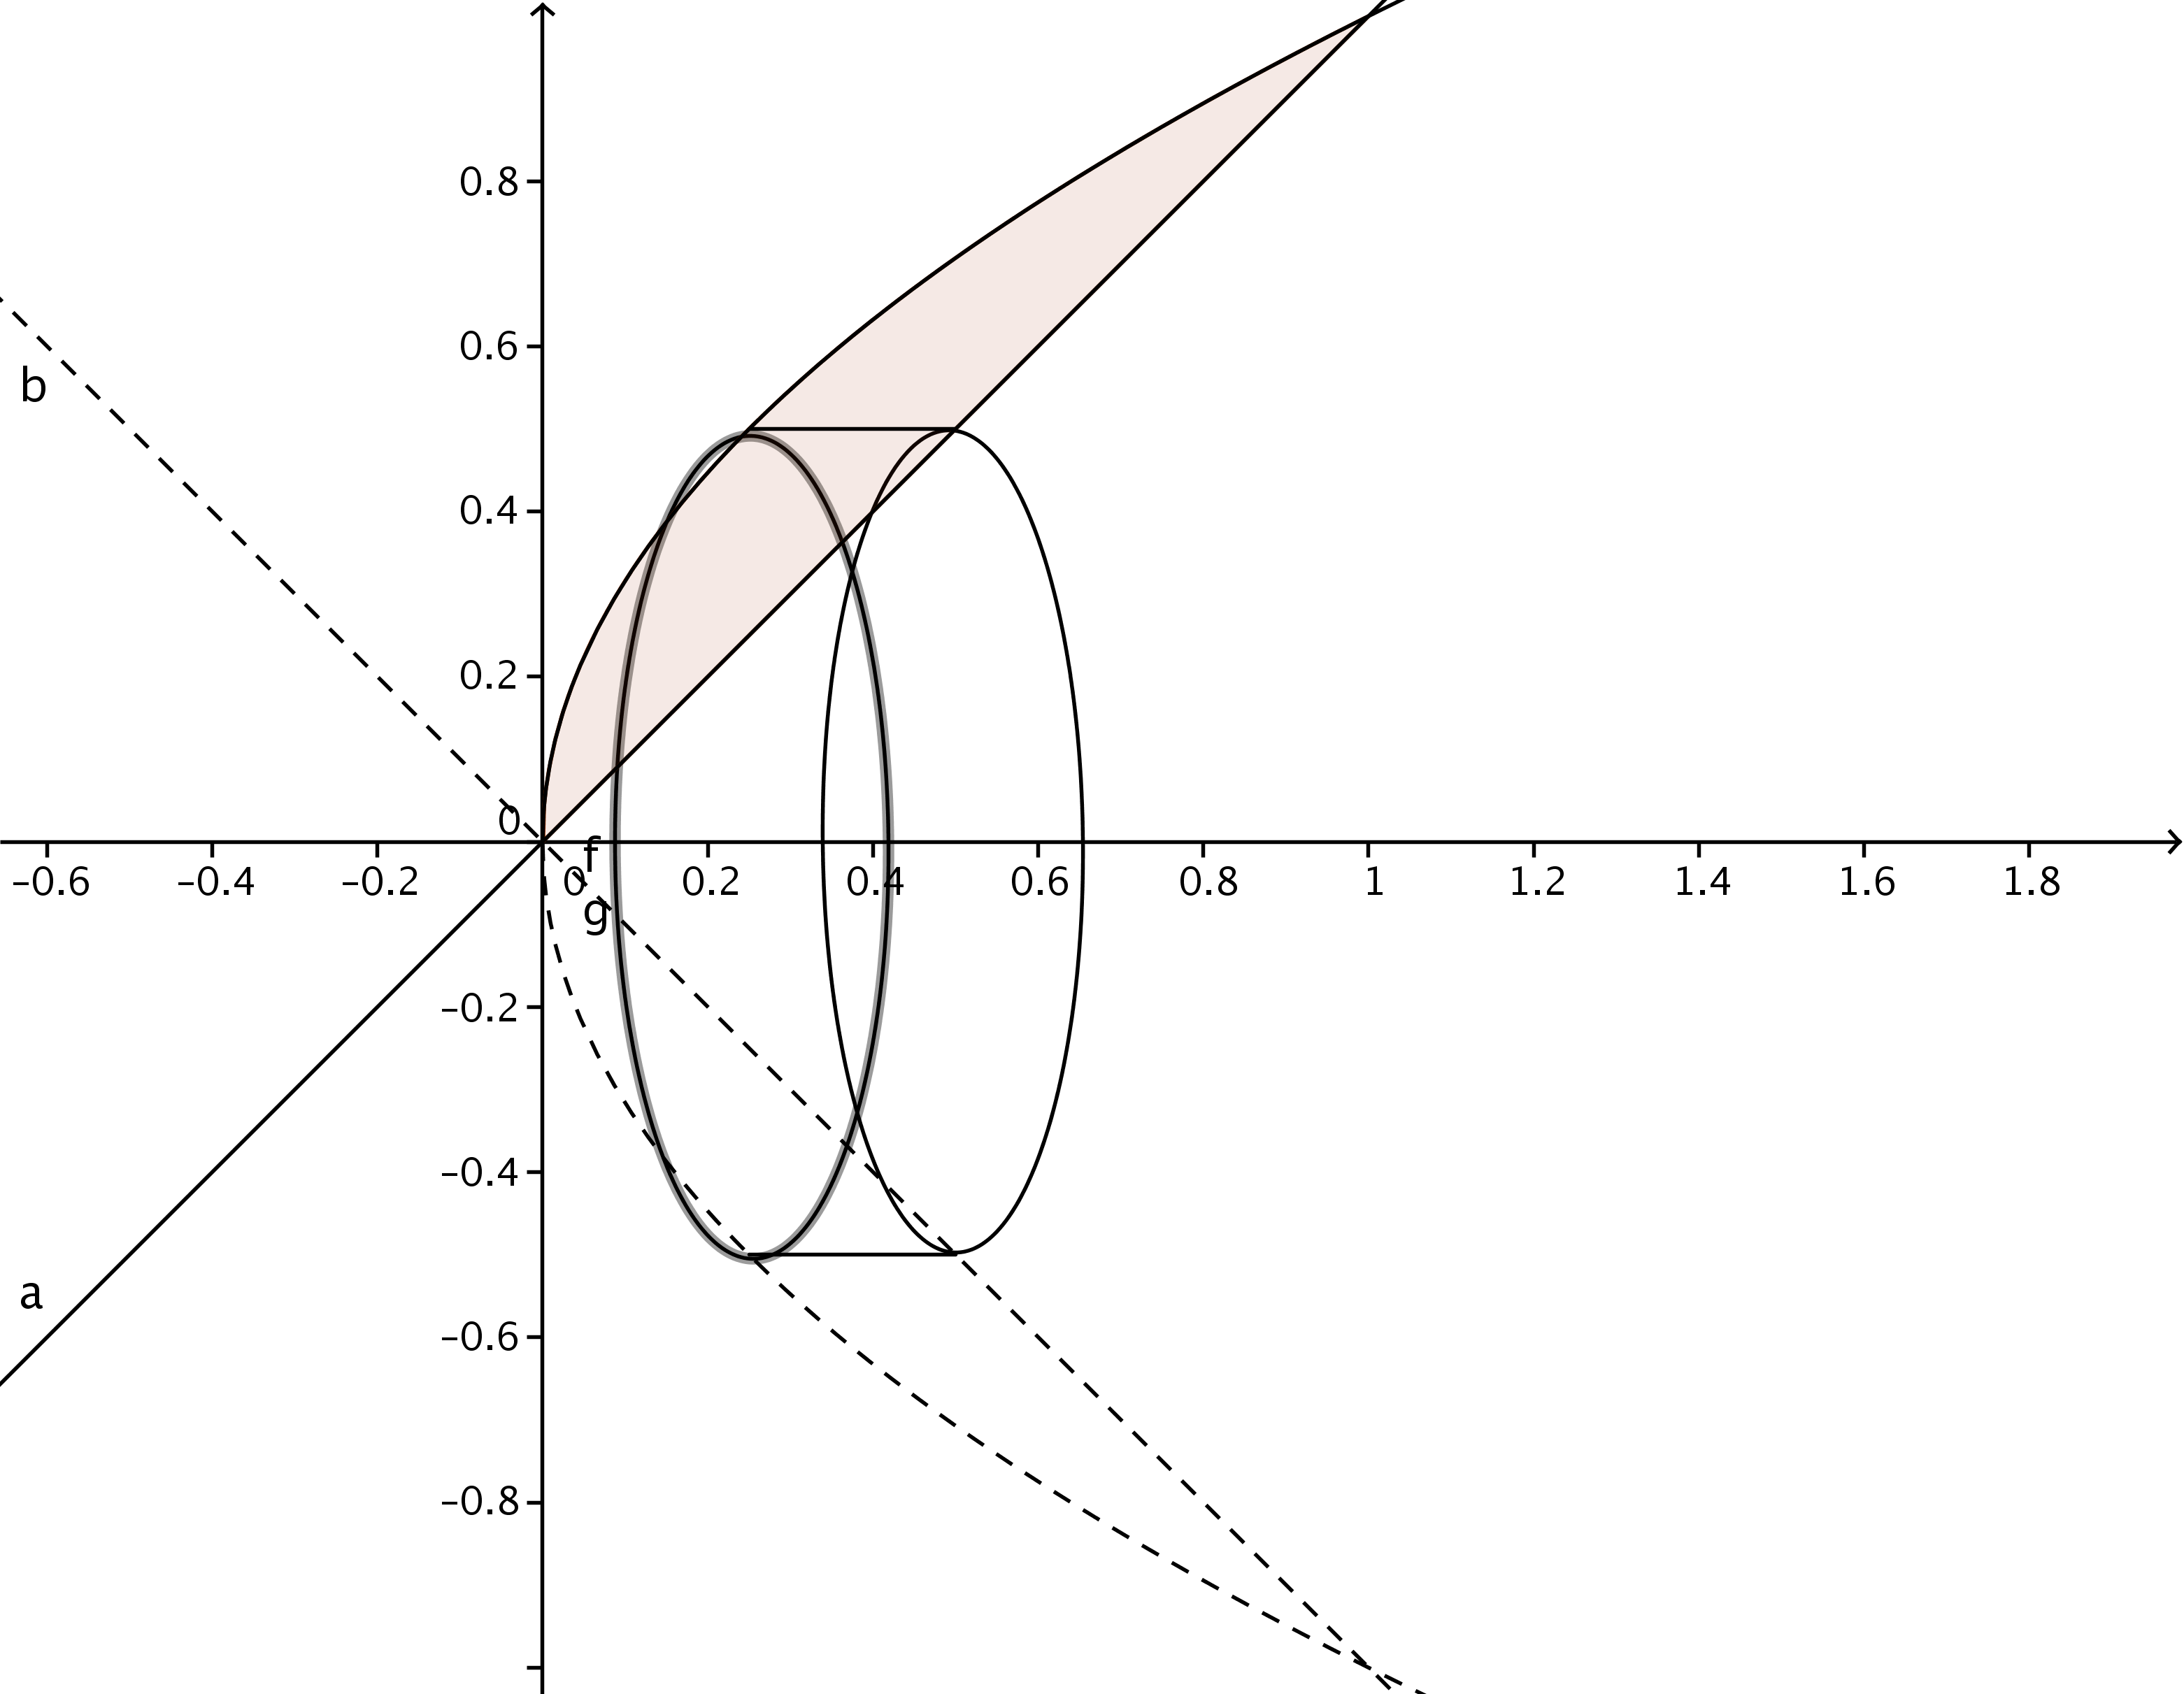
\includegraphics[width=0.5\textwidth]{WS5-6.png}
\end{center}

The graphs $y=x$ and $y=\sqrt{x}$ can be rewritten as $x=y^2$ and $x=y$. Using cylindrical shells, the radius of each cylinder is $r=y$, and the height is $h = y-y^2$, so the surface area of each shell is $2\pi y(y-y^2)$, and the volume is
\[
 V = \int_0^1 2\pi (y^2-y^3)\,dy = \frac{\pi}{6}.
\]

 \item Find the length of the curve $y=\dfrac{1}{12}x^3+\dfrac{1}{x}$, for $x\in [1,4]$.

\medskip

Arc length is given by $L=\int_a^b\sqrt{1+f'(x)^2}\,dx$, so we first compute
\begin{align*}
 1+(y')^2 & = 1+ \left(\frac{1}{4}x^2-\frac{1}{x^2}\right)^2 = 1+\left(\frac{x^4-4}{4x^2}\right)^2\\
& = 1+\frac{x^8-8x^4+16}{16x^4} = \frac{16x^4+x^8-8x^4+16}{16x^4}\\
& = \left(\frac{x^4+4}{4x^4}\right)^2.
\end{align*}
Thus, 
\[
 L = \int_0^1 \sqrt{\left(\frac{x^4+4}{4x^4}\right)^2}\,dx = \int_0^1 \left(\frac{x^4}{4}+\frac{1}{x^4}\right)\,dx = 6.
\]


 \item Find the area of the surface obtained by revolving $y=\sqrt{x}$, for $x\in [0,1]$, about the $x$-axis.

\medskip

Since we're revolving about the $x$-axis and $y$ is given as a function of $x$, we use the formula $S = 2\pi \int_a^b f(x)\sqrt{1+f'(x)^2}\,dx$. With $f(x)=\sqrt{x}$, we have
\[
 1+f'(x)^2 = 1+\left(\frac{1}{2\sqrt{x}}\right)^2 = \frac{4x+1}{4x}.
\]
The surface area is thus
\[
 S = 2\pi \int_0^1 \sqrt{x}\sqrt{\frac{4x+1}{4x}}\,dx = \pi\int_0^1 \sqrt{4x+1}\,dx = \left.\frac{\pi}{4}\cdot\frac{2}{3}(4x+1)^{3/2}\right|_0^1 = \frac{\pi}{6}(5^{3/2}-1).
\]

 \item Find the area of the surface obtained by revolving $y=x^2$, for $x\in [0,1]$, about the $y$-axis.

\medskip

This time we're revolving a function of $x$ about the $y$-axis, so we use the formula $S=2\pi\int_a^b x\sqrt{1+f'(x)^2}\,dx$. With $f(x)=x^2$ we have $f'(x)=2x$, so
\[
 S = 2\pi\int_0^1 x\sqrt{1+4x^2}\,dx = \frac{\pi}{4}\int_1^5 \sqrt{u}\,du = \frac{\pi}{6}(5^{3/2}-1),
\]
using the substitution $u=1+4x^2$, so $du=8x\,dx$, and when $x=0$, $u=1$, and when $x=4$, $u=5$. Notice that the answer is the same as the previous problem. Draw a picture for both surfaces and you'll see that this is not a coincidence.


 \item Find the area of the surface obtained by revolving $x=1+2y^2$, $1\leq y\leq 2$, about the $x$-axis.

Since we have $x$ given as a function of $y$ and we're revolving about the $x$-axis, we use the formula $S=\int_c^d y\sqrt{1+g'(y)^2}\,dy$. Here, $g(y) = 1+2y^2$, so $g'(y) = 4y$. Thus,
\[
 S = 2\pi\int_1^2 y\sqrt{1+16y^2}\,dy = \frac{\pi}{16}\int_{17}^{65}\sqrt{u}\,dy = \frac{\pi}{24}(65^{3/2}-17^{3/2}).
\]

\end{enumerate}


\end{document}